\documentclass[12pt, a4paper, oneside]{ctexart}
\usepackage{amsmath, amsthm, amssymb, bm, color, framed, graphicx, hyperref, mathrsfs, mathtools, enumerate, tikz}
\usepackage{float}
\usepackage{booktabs}
\usepackage{subcaption} 



\usetikzlibrary{patterns}

\title{\textbf{Homework 10}}
\author{萃英学院\qquad 2022级\qquad 王一鑫}
\date{\today}
\linespread{1.5}
\newcounter{problemname}
\newenvironment{problem}{\begin{framed}\stepcounter{problemname}\par\noindent\textsc{Problem \arabic{problemname}. }}{\end{framed}\par}
\newenvironment{solution}{%
	\par\noindent\textsc{Solution. }\ignorespaces
}{%
	\hfill$\qed$\par
}
\newenvironment{note}{\par\noindent\textsc{Note of Problem \arabic{problemname}. }}{\\\par}

\begin{document}
	
	\maketitle

	\begin{problem}
		(Exercise 5.19)
        
		Consider the map in Fig. \ref{fig:p1}, in which the countries are to be coloured red, blue, green and yellow.

		\begin{enumerate}
			\item[(i)] Show that country \( A \) must be red.
			\item[(ii)] What colour is country \( B \)?
		\end{enumerate}

		\begin{figure}[H]
            \small
            \centering
            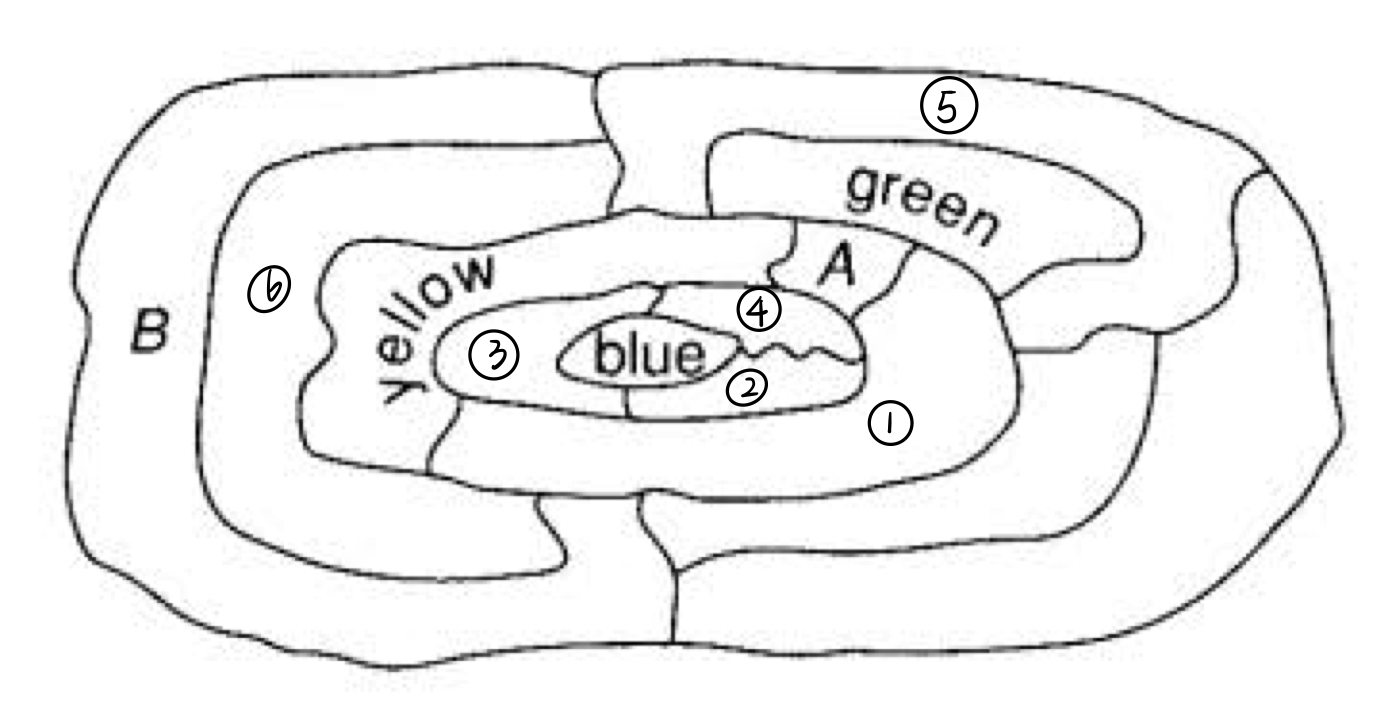
\includegraphics[width=0.66\columnwidth]{figure/fig2.jpg}
            \caption{Figure for Problem 1.}
            \label{fig:p1}
        	\end{figure}
	\end{problem}

	\begin{solution}
		\begin{enumerate}[(i)]
			\item Suppose not, then A must be blue, thus \textcircled{1} must be red, and \textcircled{3} must
				be green, \textcircled{2} must be yellow. In this way \textcircled{4} is surrounded by fore colours, which
				is a contradiction. Thus $A$ must be red.
			\item Follow the rule of colouring, we colour $A$ red, \textcircled{1} blue, \textcircled{5} red, \textcircled{6} green.
			Then $B$ must be yellow.
		\end{enumerate}
        
        

		
	\end{solution}

	\begin{problem}
        (Exercise 5.22)

        The plane is divided into a finite number of regions by drawing infinite straight lines in an arbitrary manner. 
		Show that these regions can be 2-coloured.
		
    \end{problem}
	
    \begin{solution} 
       
		We use induction on the number of lines \( n \).

		First $n = 1$. A single line divides the plane into two regions. Color one region red and the other blue. The two-coloring condition is satisfied.

		Now assume that any configuration of \( k \) lines can be 2-colored. Consider a configuration with \( k+1 \) lines. Remove one line \( L \), leaving \( k \) lines. By the inductive hypothesis, the remaining regions can be 2-colored. Reinsert \( L \). This line intersects existing regions and splits some into pairs of new regions. To maintain a valid 2-coloring, invert the color (e.g., red \(\leftrightarrow\) blue) of every region on one side of \( L \). 

		This inversion preserves distinct colors for regions separated by existing lines. For regions adjacent across \( L \), their colors differ because one side was inverted. Thus, the new configuration with \( k+1 \) lines remains properly 2-colored.

		By induction, the statement holds.

    \end{solution}

	\begin{problem}
		(Exercise 5.24)

		Let \( G \) be a simple plane graph with fewer than 12 faces, and suppose that each vertex of \( G \) has degree at least 3.

		\begin{enumerate}
			\item[(i)] Use Exercise 4.17 to prove that \( G \) is 4-colourable-(v).
			\item[(ii)] Dualize the result of part (i).
		\end{enumerate}

	\end{problem}

	\begin{solution}
		
		\begin{enumerate}[(i)]
			\item By Exercise 4.17, any simple plane graph \( G \) with fewer than 12 faces contains at least one face 
			bounded by at most four edges. 

			Let us proceed by induction on the number of vertices of \( G \).

			Suppose that every smaller plane graph with the given properties is 4-colourable. 
			Given that each vertex has degree at least 3, we use the face with at most four edges 
			to find a reducible configuration. In particular, since the graph is simple and planar, 
			and this face is bounded by at most four edges, we can remove a vertex on this face, apply the inductive 
			hypothesis to colour the smaller graph, and then extend the colouring to the removed vertex. 
			Since the vertex has at most 4 neighbours, there are always at least one of the four colours available to assign.

			Therefore, by induction, \( G \) is vertex-4-colourable. \qed
			\item 
				Consider the dual graph \( G^* \) of the plane graph \( G \). 

				Since \( G \) has fewer than 12 faces, the dual graph \( G^* \) has fewer than 12 vertices. 
				Furthermore, because \( G \) is simple and planar and each vertex in \( G \) has degree at least 3, 
				the faces of \( G \) (and hence the vertices of \( G^* \)) are bounded by cycles of length at least 3.

				By dualizing the result of part (i), we conclude that Any simple plane graph \( H \) with fewer 
				than 12 vertices, where each face is bounded by at least three edges, is 4-colourable-(f).
		\end{enumerate}

	\end{solution}

	\begin{problem}
		(Exercise 5.29)

        What is the chromatic index of each of the Platonic graphs?
        
    
	\end{problem}
    
	\begin{solution}
      
		 According to Vizing's Theorem, for any simple graph $G$, we have:
		\[
		\Delta(G) \leq \chi'(G) \leq \Delta(G) + 1,
		\]
		where $\Delta(G)$ is the maximum degree of $G$.

		\noindent\textbf{Results}

		\begin{center}
		\begin{tabular}{@{}lccc@{}}
		\toprule
		\textbf{Graph} & \textbf{Vertices} & \textbf{Max Degree} $\Delta$ & \textbf{Chromatic Index} $\chi'$ \\
		\midrule
		Tetrahedron ($K_4$) & 4 & 3 & 3 \\
		Cube & 8 & 3 & 3 \\
		Octahedron & 6 & 4 & 4 \\
		Dodecahedron & 20 & 3 & 3 \\
		Icosahedron & 12 & 5 & 5 \\
		\bottomrule
		\end{tabular}
		\end{center}
		
	\end{solution}
		

		
	
	\begin{problem}
		(Exercise 5.31)

        Prove that if \( G \) is a cubic Hamiltonian graph, then \( \chi'(G) = 3 \).

	\end{problem}
	
	\begin{solution}

		Since \( G \) is regular of degree 3, we have \( \chi'(G) \geq 3 \). 
		To obtain a 3-colouring of the edges of \( G \), we colour the edges of a Hamiltonian cycle alternately 
		red and blue, and then colour the remaining edges green.

		
	\end{solution}
	
	\begin{problem}
        (Exercise 5.32)

        \begin{enumerate}[(i)]
			\item By considering the possible 3-colourings of the outer 5-cycle, prove that the Petersen graph has chromatic index 4.
			\item Using part (i) and Exercise 5.31, deduce that the Petersen graph is non-Hamiltonian.
		\end{enumerate}


	\end{problem}
	
	\begin{solution}
		\begin{enumerate}[(i)]
			\item The colouring is shown in Fig \ref{fig:Colouring}.
			\begin{figure}[H]
            \small
            \centering
            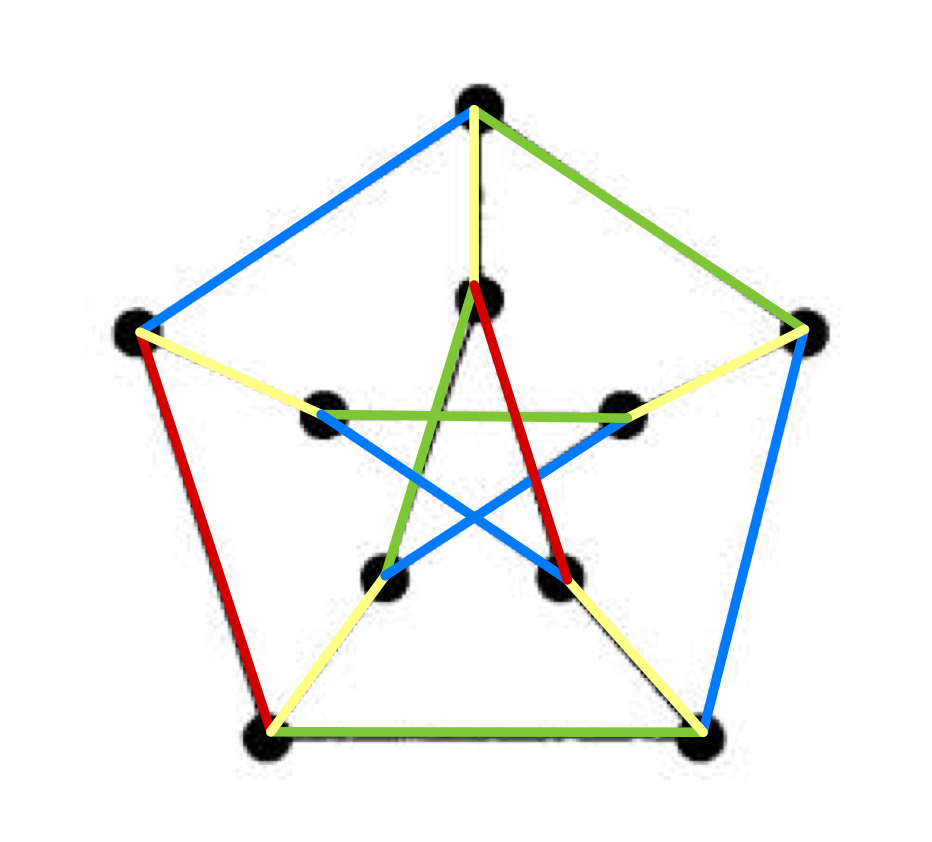
\includegraphics[width=0.4\columnwidth]{figure/fig1.jpg}
            \caption{Colouring.}
            \label{fig:Colouring}
        	\end{figure}
			\item Suppose not, by Exercise 5.31, the Petersen graph is a cubic Hamiltonian, thus
				\( \chi'(G) = 3 \), which is a contradiction with (i).
		\end{enumerate}
       
        

	\end{solution}
	
	\begin{problem}
		(Exercise 5.33)

		A graph \( G \) is \textbf{$k$-critical} if \(\chi(G) = k\) and if the deletion of any vertex yields a graph with smaller chromatic number.

		\begin{enumerate}
			\item[(i)] Find all 2-critical and 3-critical graphs.
			\item[(ii)] Give an example of a 4-critical graph.
			\item[(iii)] Prove that, if \( G \) is \( k \)-critical, then
			\begin{enumerate}
				\item[(a)] every vertex of \( G \) has degree at least \( k - 1\);
				\item[(b)] \( G \) has no cut-vertices.
			\end{enumerate}
		\end{enumerate}
	
	\end{problem}
	
	\begin{solution}
		\begin{enumerate}[(i)]
			\item A graph has chromatic number \( \chi(G) = 2 \), and the removal of any vertex must reduce the 
			chromatic number to 1. A graph with \( \chi(G) = 2 \) and this property must be a single edge: \( K_2 \).
			A minimal graph with chromatic number 3 is an odd cycle with length at least 3. All odd cycles \( C_{2n+1} \) for \( n \geq 1 \) are 3-critical.
			\item The complete graph \( K_4 \) is 4-critical. Its chromatic number is 4, and removing any vertex results in \( K_3 \), which is 3-chromatic.
			\item 
			\begin{enumerate}[(a)]
				\item  Suppose \( G \) is \( k \)-critical and assume, for contradiction, there exists a vertex \( v \) with \( \deg(v) < k-1 \). Remove \( v \); by the definition of \( k \)-criticality, the remaining graph \( G - v \) can be colored with \( k-1 \) colors. Since \( v \) has fewer than \( k-1 \) neighbors, at least one color is unused among its neighbors. Assign this color to \( v \), resulting in a proper \( (k-1) \)-coloring of \( G \), contradicting \( \chi(G) = k \). Hence, every vertex must have degree \( \geq k-1 \).
				\item  Assume \( G \) is \( k \)-critical and contains a cut-vertex \( v \). Removing \( v \) disconnects \( G \) into components \( C_1, C_2, \ldots, C_m \). Each \( C_i \) can be colored with \( k-1 \) colors. Since \( v \) is adjacent to vertices in disjoint components, color \( v \) with a color distinct from all its neighbors in every \( C_i \). This produces a \( (k-1) \)-coloring of \( G \), contradicting \( \chi(G) = k \). Therefore, \( G \) cannot have cut-vertices.
			\end{enumerate}
		\end{enumerate}
	\end{solution}

	\begin{problem}
        (Exercise 5.34) 
        
		Generalize the results of Exercise 5.8 to the cases where
		\begin{enumerate}[(i)]
			\item \( G \) has girth \( r \),
			\item \( G \) has thickness \( t \).
		\end{enumerate}

	\end{problem}
	
	\begin{solution}
     
         \begin{itemize}
            \item[(i)] 
					We first consider the case where \( G \) is a simple planar graph of girth \( r \), 
					that is, the length of the shortest cycle in \( G \) is at least \( r \). 

					Let \( v, e, f \) denote the number of vertices, edges, and faces of \( G \), 
					respectively. By Euler’s formula for planar graphs,
					\[
					v - e + f = 2.
					\]
					Since \( G \) has girth \( r \), every face of \( G \) is bounded by at least \( r \) edges. 
					Each edge is counted in at most two face boundaries, hence
					\[
					rf \leq 2e \quad \Rightarrow \quad f \leq \frac{2e}{r}.
					\]
					Substituting this bound into Euler’s formula yields:
					\[
					v - e + \frac{2e}{r} \geq 2 \quad \Rightarrow \quad v \geq e \left(1 - \frac{2}{r}\right) + 2.
					\]
					Solving for \( e \) in terms of \( v \), we obtain:
					\[
					e \leq \frac{r}{r - 2}(v - 2).
					\]
					Now consider the average degree \( \bar{d} \) of the graph:
					\[
					\bar{d} = \frac{2e}{v} \leq \frac{2r}{r - 2} \left(1 - \frac{2}{v}\right).
					\]
					This shows that the average degree is strictly less than \( \frac{2r}{r - 2} \), 
					hence there exists at least one vertex whose degree does not exceed 
					\( \left\lfloor \frac{2r}{r - 2} \right\rfloor -1\). Thus, any simple planar graph of girth 
					\( r \) contains a vertex of degree at most \( \left\lfloor \frac{2r}{r - 2} \right\rfloor - 1 \).

					This fact enables an inductive coloring strategy. Suppose that all such graphs on fewer than 
					\( v \) vertices are \( \left\lfloor \frac{2r}{r - 2} \right\rfloor \)-colorable. 
					Let \( G \) be a graph with \( v \) vertices, and let \( v_0 \in V(G) \) be a vertex of degree 
					at most \( \left\lfloor \frac{2r}{r - 2} \right\rfloor - 1\). Then \( G - v_0 \) is a planar graph 
					of girth at least \( r \), and by the inductive hypothesis, it is 
					\( \left\lfloor \frac{2r}{r - 2} \right\rfloor \)-colorable. Since \( v_0 \) has at most 
					\( \left\lfloor \frac{2r}{r - 2} \right\rfloor -1 \) neighbors, its color can be chosen from the 
					\( \left\lfloor \frac{2r}{r - 2} \right\rfloor \) available colors to avoid conflict. 
					Hence \( G \) is \( \left\lfloor \frac{2r}{r - 2} \right\rfloor \)-colorable.

            \item[(ii)]
					We now consider the case where \( G \) is a graph of thickness \( t \). 
					That is, \( G \) can be decomposed into \( t \) planar subgraphs \( G_1, G_2, \dots, G_t \) 
					such that
					\[
					G = G_1 \cup G_2 \cup \dots \cup G_t,
					\]
					and each \( G_i \) is a planar subgraph. By the Four Color Theorem, each \( G_i \) is 4-colorable. 
					Let us assign each planar subgraph \( G_i \) a distinct color palette consisting of four unique 
					colors. In particular, define the color classes for each \( G_i \) to be disjoint: for example, 
					use colors \( \{4(i-1)+1, 4(i-1)+2, 4(i-1)+3, 4(i-1)+4\} \) for \( G_i \). 
					Then, color each \( G_i \) independently using its own palette. Since each edge lies in only one 
					of the \( G_i \), and the palettes are disjoint, adjacent vertices in \( G \) will always receive 
					distinct colors. Therefore, this strategy yields a proper coloring of \( G \) using \( 4t \) colors.

					Hence, any graph of thickness \( t \) is \( 4t \)-colorable.
            
        \end{itemize}
		
	\end{solution}


	\begin{problem}
		(Exercise 5.37)

        \begin{enumerate}[(i)]
			\item Let \( G \) be a simple graph which is not a null graph. Prove that \( \chi'(G) = \chi(L(G)) \), where \( L(G) \) is the line graph of \( G \).
			\item By combining part (i) with Brooks's theorem, prove Vizing's theorem in the case \( \Delta = 3 \).
		\end{enumerate}

          
        
    \end{problem}

	\begin{solution}
        \begin{enumerate}
			\item[(i)]	Let \( G \) be a simple graph which is not a null graph, and let \( L(G) \) denote 
			its line graph. By definition, each vertex in \( L(G) \) corresponds to an edge in \( G \), 
			and two vertices in \( L(G) \) are adjacent if and only if their corresponding edges in \( G \) 
			share a common vertex. Therefore, a proper vertex coloring of \( L(G) \) is equivalent to 
			a proper edge coloring of \( G \), where adjacent edges (i.e., edges incident to a common vertex) 
			receive different colors. It follows that the chromatic number of \( L(G) \), denoted \( \chi(L(G)) \), 
			equals the chromatic index of \( G \), denoted \( \chi'(G) \). Hence, \( \chi'(G) = \chi(L(G)) \).
			\item[(ii)] Suppose now that \( G \) is a simple graph with maximum degree \( \Delta(G) = 3 \). 
			From part (i), we know that \( \chi'(G) = \chi(L(G)) \). Since each edge in \( G \) is incident to 
			at most two vertices of degree at most three, each corresponding vertex in \( L(G) \) has degree 
			at most four. Therefore, \( \Delta(L(G)) \leq 4 \). 

			To apply Brooks's theorem, we must consider whether \( L(G) \) is a complete graph or an odd cycle. 
			If \( L(G) \) is neither, then Brooks's theorem gives \( \chi(L(G)) \leq \Delta(L(G)) \leq 4 \). 
			Since \( \chi'(G) = \chi(L(G)) \), we conclude \( \chi'(G) \leq 4 \). Moreover, since the chromatic 
			index of a graph is always at least its maximum degree, we have \( \chi'(G) \geq \Delta(G) = 3 \). 
			Hence, \( \chi'(G) \in \{3, 4\} \), which is precisely the statement of Vizing's theorem in the case 
			\( \Delta = 3 \).

			If \( L(G) \) were a complete graph \( K_5 \), then \( \chi(L(G)) = 5 \), contradicting the assumption 
			that \( \Delta(G) = 3 \), because \( L(K_4) = K_6 \) and not \( K_5 \). Thus, \( L(G) \) cannot be 
			a complete graph on five vertices. Similarly, \( L(G) \) cannot be an odd cycle because the structure 
			of a line graph derived from a simple graph with \( \Delta = 3 \) cannot form an odd cycle unless \( G \) 
			has a very specific and constrained form, which is not possible under general assumptions. 
			Therefore, the use of Brooks's theorem is valid, and Vizing's theorem holds for all simple graphs with 
			\( \Delta = 3 \).

		\end{enumerate}

    \end{solution}
		
    
	\begin{problem}
		(Exercise 5.39)

		\begin{enumerate}[(i)]
			\item Prove that, if a toroidal graph is embedded on the surface of a torus, then its faces can be coloured with seven colours.
			\item Find a toroidal graph whose faces cannot be coloured with six colours.
		\end{enumerate}

          
    \end{problem}

	\begin{solution}
       
        \begin{enumerate}[(i)]
		\item
		Let $G$ be a graph embedded on the torus. A face colouring of $G$ corresponds to a proper vertex colouring 
		of its dual graph $G^*$, where each vertex in $G^*$ represents a face of $G$, and two vertices in $G^*$ are 
		adjacent if and only if the corresponding faces in $G$ share a common edge. Since $G$ is embedded on the torus, 
		its dual $G^*$ is also embeddable on the torus. It is a classical result in topological graph theory that every 
		graph embeddable on the torus has vertex chromatic number at most seven. Therefore, the dual graph $G^*$ is 
		7-colourable, and consequently, the faces of $G$ can be properly coloured with at most seven colours.

		\item
		To construct a toroidal graph whose faces cannot be coloured with only six colours, consider the complete graph $K_7$. It is known that $K_7$ can be embedded on the torus without edge crossings. In such an embedding, the dual graph $K_7^*$ corresponds to a map with seven faces, where each face is adjacent to all others, forming a complete graph on seven vertices. Hence, the dual graph is $K_7$, which requires seven colours for a proper vertex colouring. Consequently, the original embedding of $K_7$ on the torus forms a toroidal graph whose faces require seven distinct colours, and no proper face colouring with only six colours is possible.

		\end{enumerate}
		
	\end{solution}


	
     

    

\end{document}


